\section{Schwarm-Topologien}
\index{Schwarm-Topologie}
Zum Bestimmen der sozialen Komponente des Geschwindigkeitsvektors
kommen verschiedene Topologien oder Nachbarschaftsbeziehungen zur
Anwendung. Diese Beziehungen unter den Partikeln haben einen essentiellen
Einfluss auf den Algorithmus. Generell kann zwischen gbest (global best)
und lbest (local best) unterschieden werden.

\begin{figure}[htbp]
	\centering
	\begin{minipage}{4cm}
		\centering
		%\input{partikelschwarm/gbest}
		\includegraphics{partikelschwarm/gbest-crop.pdf}\\
		GBest
	\end{minipage}
	\begin{minipage}{4cm}
		\centering
		%\documentclass{standalone}

\usepackage{tikz}
\usetikzlibrary{arrows,decorations.pathmorphing,positioning,fit,petri}
\usetikzlibrary{calc,intersections,through,backgrounds,graphs}
\usetikzlibrary{patterns,decorations.pathreplacing}

\begin{document}


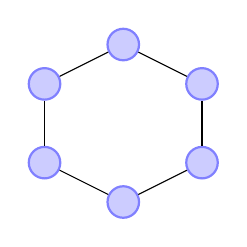
\begin{tikzpicture}
	% Styles
	[
	place/.style={circle,draw=blue!50,fill=blue!20,thick, inner sep=0pt,minimum size=4mm},
	]
                      
	% Nodes
	\node at (0,0.5)	(p1)	[place] {};
	\node at (0,1.5)	(p2)	[place] {};
	\node at (1,0)		(p3)	[place] {};
	\node at (1,2)		(p4)	[place] {};
	\node at (2,0.5)	(p5)	[place] {};
	\node at (2,1.5)	(p6)	[place] {};
	
	% Connections
	\graph[use existing nodes] {
		p1 -- p2 -- p4 -- p6 -- p5 -- p3 -- p1;
	};
	

\end{tikzpicture}

\end{document}
		\includegraphics{partikelschwarm/lbest-ring-crop.pdf}\\
		LBest - Ring
	\end{minipage}
	\begin{minipage}{4cm}
		\centering
		%\documentclass{standalone}

\usepackage{tikz}
\usetikzlibrary{arrows,decorations.pathmorphing,positioning,fit,petri}
\usetikzlibrary{calc,intersections,through,backgrounds,graphs}
\usetikzlibrary{patterns,decorations.pathreplacing}

\begin{document}

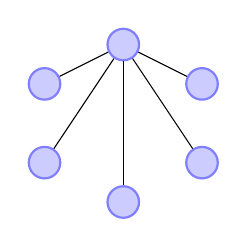
\begin{tikzpicture}
	% Styles
	[
	place/.style={circle,draw=blue!50,fill=blue!20,thick, inner sep=0pt,minimum size=4mm},
	]
                      
	% Nodes
	\node at (0,0.5)	(p1)	[place] {};
	\node at (0,1.5)	(p2)	[place] {};
	\node at (1,0)		(p3)	[place] {};
	\node at (1,2)		(p4)	[place] {};
	\node at (2,0.5)	(p5)	[place] {};
	\node at (2,1.5)	(p6)	[place] {};
	
	% Connections
	\graph[use existing nodes] {
		p4 -- p1;
		p4 -- p2;
		p4 -- p3;
		p4 -- p5;
		p4 -- p6;
	};
	

\end{tikzpicture}

\end{document}
		\includegraphics{partikelschwarm/lbest-wheel-crop.pdf}\\
		LBest - Wheel
	\end{minipage}
	\begin{minipage}{4cm}
		\centering
		%\documentclass{standalone}

\usepackage{tikz}
\usetikzlibrary{arrows,decorations.pathmorphing,positioning,fit,petri}
\usetikzlibrary{calc,intersections,through,backgrounds,graphs}
\usetikzlibrary{patterns,decorations.pathreplacing}

\begin{document}

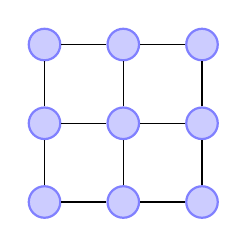
\begin{tikzpicture}
	% Styles
	[
	place/.style={circle,draw=blue!50,fill=blue!20,thick, inner sep=0pt,minimum size=4mm},
	]
                      
	% Nodes
	\node at (0,0)	(p1)	[place] {};
	\node at (0,1)	(p2)	[place] {};
	\node at (0,2)	(p3)	[place] {};
	\node at (1,0)	(p4)	[place] {};
	\node at (1,1)	(p5)	[place] {};
	\node at (1,2)	(p6)	[place] {};
	\node at (2,0)	(p7)	[place] {};
	\node at (2,1)	(p8)	[place] {};
	\node at (2,2)	(p9)	[place] {};
	
	% Connections
	\graph[use existing nodes] {
		p1 -- p2 -- p3;
		p4 -- p5 -- p6;
		p7 -- p8 -- p9;
		p1 -- p4 -- p7;
		p2 -- p5 -- p8;
		p3 -- p6 -- p9;
	};

\end{tikzpicture}

\end{document}

		\includegraphics{partikelschwarm/lbest-neumann-crop.pdf}\\
		LBest - Von Neumann
	\end{minipage}
	\caption{Schwarm-Topologien}
	\label{schwarm-topologien}
\end{figure}

\subsection{GBest}
\index{GBest}
Die gbest Topologie geht von einem transparentem Partikelschwarm aus,
in welchem die jeweils pers"onlich besten Positionen aller Partikel
bekannt sind. Die soziale Komponente des gesamten Schwarms bildet sich
also aus dem Abstand zur besten Position des gesamten Schwarms. Ein
Vorteil dieser Nachbarschaftsbeziehung ist, dass der Schwarm schnell
konvergiert, weil alle Partikel auf die momentan beste Position zulaufen.

\subsection{LBest}
\index{LBest}
Es existieren mehrere verschiedene lbest Architekturen. Die verbreitetsten
Architekturen sind in Abbildung \ref{schwarm-topologien} dargestellt. Das
Grundprinzip von lbest ist, dass jedes Partikel nur auf die besten
Positionen seiner Nachbarn zugreifen kann. Wie die Nachbarpartikel
bestimmt werden ist von der gew"ahlten Topologie abh"angig. Die lbest
Methode hat den Vorteil, dass die Wahrscheinlichkeit gegen ein lokales
Optimum zu konvergieren bedeutend kleiner ist. Daf"ur dauert es im
Normalfall l"anger, ein Optimum zu finden, als mit der gbest Methode.

In der Natur kommunizieren Schwarmtiere mit ihren n"achsten Nachbarn. Bei
jeder Iteration die Nachbarn zu bestimmen w"are jedoch ein grosser
Rechenaufwand, welcher erfahrungsgem"ass nicht n"otig ist. Meist werden
heute bei der Initialisierung die Nachbarn bestimmt und diese bleiben
w"ahrend der Laufzeit dieselben.

\subsection{Wahl der Topologie}
Die Wahl der Topologie h"angt stark von der Problemstellung ab. Es
lassen sich leider keine generellen Aussagen machen, wann genau welche
Topologie ideal ist. Wie erw"ahnt konvergieren Partikelschw"arme nach
gbest Topologie schneller gegen ein Optimum, w"ahrend lbest Schw"arme
weniger gegen lokale Optima konvergieren.

\subsection{Subpopulationen}
Um die Vorteile beider Topologien zu vereinen, kann das von genetischen
Algorithmen (GA) bekannte Prinzip der Subpopulationen verwendet
werden. Dabei wird der eigentliche Schwarm in mehrere Subpopulationen
unterteilt, welche unabh"angig von einander die PSO ausf"uhren. Oft werden
Subpopulationen verwendet, um einzelne Teilgebiete genauer untersuchen
zu k"onnen.


\subsubsection{Hierarchische Subpopulationen}
Ein Spezialfall der Partikelschwarm-Optimierung ist
die \textit{hierarchical subpopulation PSO} (HS-PSO)
\cite{ChuanLin-HSPSO}. Das Prinzip der HS-PSO ist die Unterteilung des
Schwarms nach einem hierarchischen Prinzip, wie zum Beispiel in einer
Unternehmung.

\begin{figure}[htbp]
	\centering
	%\documentclass{standalone}

\usepackage{tikz}
\usetikzlibrary{arrows,decorations.pathmorphing,positioning,fit,petri}
\usetikzlibrary{calc,intersections,through,backgrounds,graphs}
\usetikzlibrary{patterns,decorations.pathreplacing}

\begin{document}

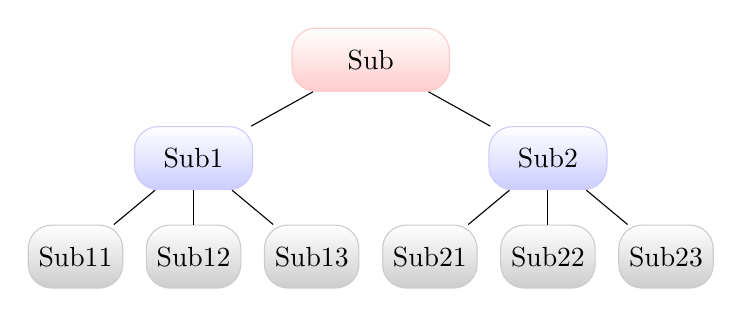
\begin{tikzpicture}
	% Styles
	[
	sub/.style={rectangle, rounded corners=3mm, minimum size=8mm, minimum width=1.2cm, draw=black!20, top color=white, bottom color=black!20},
	mid/.style={rectangle, rounded corners=3mm, minimum size=8mm, minimum width=1.5cm, draw=blue!20, top color=white, bottom color=blue!20},
	top/.style={rectangle, rounded corners=3mm, minimum size=8mm, minimum width=2cm, draw=red!20, top color=white, bottom color=red!20}
	]
                      
	% Nodes
	\node at (3.75,2.5)	(sub)	[top] {Sub};
	\node at (1.5,1.25)	(sub1)	[mid] {Sub1};
	\node at (6,1.25)	(sub2)	[mid] {Sub2};
	\node at (0,0)		(sub11)	[sub] {Sub11};
	\node at (1.5,0)	(sub12)	[sub] {Sub12};
	\node at (3,0)		(sub13)	[sub] {Sub13};
	\node at (4.5,0)	(sub21)	[sub] {Sub21};
	\node at (6,0)		(sub22)	[sub] {Sub22};
	\node at (7.5,0)	(sub23)	[sub] {Sub23};
	
	% Connections
	\graph[use existing nodes] {
		sub -- sub1;
		sub -- sub2;
		sub1 -- sub11;
		sub1 -- sub12;
		sub1 -- sub13;
		sub2 -- sub21;
		sub2 -- sub22;
		sub2 -- sub23;
	};

\end{tikzpicture}

\end{document}
	\includegraphics{partikelschwarm/hs-pso-crop.pdf}\\
	\caption{Hierarchical Subpopulation PSO}
	\label{hs-pso}
\end{figure}

Die besten Partikel der Subpopulationen \textit{Sub11} - \textit{Sub13}
bilden zusammen die Population \textit{Sub1}. Die besten Partikel der
Populationen \textit{Sub1} - \textit{Sub2} bilden den Hauptschwarm
\textit{Sub}.

Die einzelnen Partikelschw"arme lassen sich unterschiedlich
konfigurieren. So schl"agt Chuan Lin in \cite{ChuanLin-HSPSO} vor,
Schw"arme in tiefen Hierarchiestufen auf das Erforschen des Gesamtgebiets
einzustellen (d.h. geringe Sozialkomponente), w"ahrend die h"oheren
Hierarchiestufen relativ tr"age sind. Damit l"asst sich ein grosses Gebiet
erforschen, doch der Schwarm konvergiert kaum gegen lokale Minima.

In Benchmark-Tests haben HS-PSO Varianten bedeutend bessere Resultate als
herk"ommliche gbest und lbest Topologien hervorgebracht. Das Thema ist
jedoch erst schwach erforscht. Weitere Arbeiten, vor allem zu adaptiven
hierarchischen Strukturen und dem Informationsaustausch zwischen den
Subpopulationen sind jedoch angek"undigt.

